% begin module tangents-ex1
\begin{frame}
\begin{example} %[Example 1, p. 136]
Find an equation for the tangent line to the parabola $y = x^2$ at the point $P = (1,1)$.

\begin{columns}[c]
\column{.4\textwidth}
\psset{xunit=0.8cm, yunit=0.8cm}
\begin{pspicture}(-1,-0.5)(2.6,6.4)
\psframe*[linecolor=white](-1,-0.5)(2.6,6.4)
\psaxes[ticks=none, labels=none]{<->}(0,0)(-1,-0.5)(2.5,4.5)
\tiny
\psLabelXOne
\psLabelYOne
\rput[l](0.2, 3.5){$y=x^2$}
%Function formula: (x)^{2} 
\psplot[linecolor=red, plotpoints=1000]{-1}{2.5}{x 2 exp }
\psline[linecolor=blue](0.25, -0.5)(2.5,4)
\psFullDotBlack{1}{1}
\rput[lt](1.1, 0.9){$P=(1,1)$}
\end{pspicture}
%\ \uncover<9->{%
%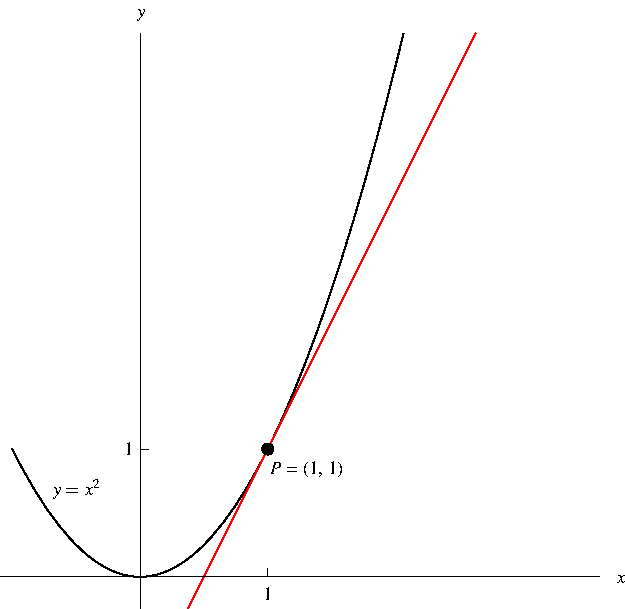
\includegraphics[height=4.5cm]{derivatives/pictures/02-01-secanta.pdf}%
%}%
\column{.6\textwidth}
\uncover<2->{%
Here $a = 1$ and $f(x) = x^2$.
}%
\abovedisplayskip=0pt
\belowdisplayskip=0pt
\abovedisplayshortskip=0pt
\belowdisplayshortskip=0pt
\begin{align*}
\uncover<3->{m} & \uncover<3->{ = }  \uncover<3->{\lim_{x\rightarrow 1} \frac{f(x)-f(1)}{x-1}}\\
& \uncover<4->{ = }  %
\uncover<4->{\lim_{x\rightarrow 1}\frac{x^2 - 1}{x-1}}\\
& \uncover<5->{ = }  %
\uncover<5->{\lim_{x\rightarrow 1}\frac{(x - 1)(x+1)}{x-1}}\\
& \uncover<6->{ = }  %
\uncover<6->{\lim_{x\rightarrow 1}(x+1)}\uncover<7->{ = 1 + 1 = 2}
\end{align*}
\uncover<8->{
Point-slope form: $y - 1 = 2(x - 1)$, or $y = 2x - 1$.
}
\end{columns}
\end{example}
\end{frame}
% end module tangents-ex1
